\documentclass[11pt]{article}
\usepackage[T1]{fontenc}
\usepackage[latin1]{inputenc}
\usepackage{enumerate}
\usepackage{setspace}
\usepackage{amsmath,amssymb,amsthm}
\usepackage{graphicx}
\usepackage{bbm}
\usepackage[round]{natbib}
\usepackage[nohead]{geometry}
\usepackage[bottom]{footmisc}
\usepackage{indentfirst}
\usepackage{endnotes}
\usepackage{graphicx}%
\usepackage{eurosym}
\usepackage{array}
\usepackage{booktabs}
\usepackage{caption}
\usepackage{subcaption}
% \usepackage[hidelinks]{hyperref}
\usepackage{floatrow} %[capposition=top]
\floatsetup{footposition=bottom,capposition=top}
\renewcommand{\labelitemi}{--}
\renewcommand{\labelitemii}{$\bullet$}
\bibliographystyle{chicago}
% \geometry{left=1in,right=1in,top=1.00in,bottom=1.0in}
\let\olditemize\itemize
\renewcommand{\itemize}{
  \olditemize
  \setlength{\itemsep}{-1pt}
}

\begin{document}

\title{Creation of a low cost branch by a major retailer: Evidence from the French gasoline market\ \\ \ \\(Very preliminary)}
\author{Etienne Chamayou\thanks{e-mail:
\textit{etienne.chamayou@ensae.fr}}\medskip\\{\normalsize CREST and Department of Economics, Ecole Polytechnique }}
\maketitle

\sloppy%

\onehalfspacing

\textbf{Abstract:}

Total S.A is one of the five "Supermajor" oil companies in the world and operates the largest gas station network in France. End of 2011, the company has launched a new brand, "Total Access", with the stated goal of recapturing market shares lost due to the development of supermarket gas station networks. The change in pricing policy and its impact on competition is studied using daily price data obtained from a comparison website. Empirical evidence confirms that the proximity of supermarkets is a major determinant in re-branding choices made by Total, and that converted gas stations are able to post prices in line with supermarket gas stations. Changes at competitors' are measured with difference-in-difference and discontinuity regressions. While 80\% of competitors do not appear to alter their pricing policy, the remaining 20\% exhibit upwards and downwards adjustments in equal proportions. [TODO: explanation of reaction: no reaction because tough competition before? downward reaction for supermarkets vs. upward for independent and oil?

\strut

\textbf{Keywords:} Competition, Gasoline

\strut

\textbf{JEL Classification Numbers:} L13

\pagebreak%
%\doublespacing

\section{Introduction}

Describe creation of Total Access, mention how cut in price is detected, data available, literature?

\section{Literature}

Relevant literature? Rather theoretical: standard model predictions... what about similar empirical observations?

\section{The French retail gasoline market}

\subsection{Information source overview}

As is put by the 2011 governmental report on the French retail gasoline market, "nobody knows precisely the number of gas stations operating in the markets". Consequently, any investigation of competition in the French retail gasoline market starts with a difficult quest for trustworthy information. The following section offers a brief overview of the available information sources and of their limits.

Two websites relying on crowdsourcing i.e information provided by users, Carbeo and Zagaz, were launched respectively in 2005 and 2006. In 2007, a decree was implemented making it mandatory for gas stations having sold over 500m$^{3}$ gas the previous year to keep prices posted on the governmental website prix-carburants.economie.gouv.fr. The 2011 governmental report notes that shortly after its launch the website started being scraped in a significant way, to the extent that user experience was deteriorated. In 2009, as a consequence, licenses were created to allow for resale of price data for internal or commercial use.

The launch of the governemental website exercised significant pressure on the young websites Zagaz and Carbeo. Zagaz still exists and has stuck to its pure crodwsourcing philosophy. Carbeo, on the contrary, purchased a licence from the governement as early as 2009. Interestingly, in 2011, the governemental body in charge of town and country planning worked with Zagaz data to study the French retail gas station network. Zagaz most likely remains the most comprehensive source of information but suffers from a lack of users in many regions.

\subsection{Retail gasoline distribution}

The size of the French gas station network has been decreasing at a steady pace over the last decades, from c. 40,000 in 1980 to c. 12,000 currently, mainly as a result of increased car capacities.  A strong competitive pressure has furthermore been generated by supermarkets progressively penetrating the market. They currently represent c. 50\% of sales in retail gasoline.

As of May 20, 2014, Zagaz lists c. 12,832 gas stations, but no price was recorded over the last months/years for many of them so that this figure most certainly overestimates the actual number of gas stations. In April 2013, UFIP quoted the numbers of 11,662 (4,947 supermarkets and 6,715 "traditional" players) for 2012 and 11,476 for 2013 (4,979 supermarkets and 6,497 "traditional" players, source: Nielsen). UFIP also reported that 1,506 gas stations sold less than 500m$^{3}$ in 2012 (1,433 in 2013), with the median gas station selling between 1,000 and 3,000m$^{3}$ (same for 2013).

Gas stations are essentially either owned and operated by a chain or with a "location-gerance" contract according to which the manager receives a commission on gasoline sold (e.g. only 200 gas stations set prices independently among gas stations from Total brand). There is significant evidence that many gas stations hardly make any profits: oil companies exiting the market (Shell and BP), drastically reducing the size of their organic network (Esso), bankrupts or terminations of independent gas stations etc.

Key cost components are the cost of wholesale gasoline, including delivery fees,  gas station operating expenses, and taxes. Taxes included a fix part called TICPE, which slightly varies between regions, and the classical Value-Added Tax (19.6\% over the period studied, which bear on cost and TICPE).

\subsection{Diesel consumption}

Diesel consumption currenlty accounts for c. 80\% of total gasoline consumption. A signicant increase in the diesel share was achieved over the last decades through a lower tax on diesel. At a very aggregate level, two kinds of consumers can be distinguished: businesses and individual customers. Businesses are typically offered card programs which allow them to monitor employees' consumptions and obtain rebates. An important implication is that the price of the gas station is irrelevant (or only partly relevant) to a significant number of transations in the market.
Consumers can get information about prices from a variety of sources: at gas stations, on their gps, on mobile phone applications (e.g. Zagaz, Carbeo, Essence Free) and on a computer or mobile phone browser (Prix-Carburants.gouv.fr).

\section{Data}

\subsection{Data overview}

Data about daily diesel prices, gas station locations, opening hours and amenities were collected from website prix-carburants.gouv.fr. Gas station location was verified and improved with data from Zagaz (information provided by users about gas station locations was observed to be of better quality) and OpenStreetMap. Finally, the gas station database was merged with INSEE data in order to add information about local markets (rural/center/suburb, population, car equipment etc.). Rotterdam wholesale diesel price is used as proxy for gas stations' variable costs.

\subsection{Context of studied period}

The period covered is marked by two significant events of different natures. One is a change of pricing strategy by a leading retail brand affecting the whole country and the other is a governmental intervention.

The first event is the progressive conversion by the oil company "Total" of c. 600 of its gas stations to low cost gas stations branded "Total Access" i.e. gas stations whose prices are aligned with supermarket gas stations. About half the conversions occur during the period covered by the paper. Though these conversions are obviously not heterogeneous shocks to the market, they yet involve a significant number of gas stations lowering their price by c. 10 Euro cents per liter virtually overnight.

The second event is of political nature. On August 29, 2012, a decrease in price of 6 Euro cents per litre was announced by the government, following an election promise made by Francois Hollande. This decrease was (to be) achieved by a decrease of tax of 3 Euro cents per litre and an equivalent "effort" by gas station operators. Also, it must be noted that a small portion of the tax on gasoline is set by regions on an annual basis.

\subsection{Descriptive statistics}

\subsubsection{Retail price vs. wholesale cost of diesel}

Descriptive statistics are provided for a period of 640 days starting September 9, 2011 and ending May 6, 2013. Four subperiods of data are yet missing for various technical reasons, thus reducing the number of observed days to 564\footnote{Respective day lengths of missing subperiods are 11 (2012/07/08-2012/07/18), 10 (2012/08/13-2012/08/22), 49 (2012/12/04-2013/01/21) and 6 (2013/04/04-2013/04/09).}. The end of the period studied has been determined arbitrarily to avoid including another missing subperiod and to keep the database to a reasonable size.

\begin{figure}[!h]
    \caption{Diesel prices and retail gross margin (09/2011-06/2013)}
	\centering
		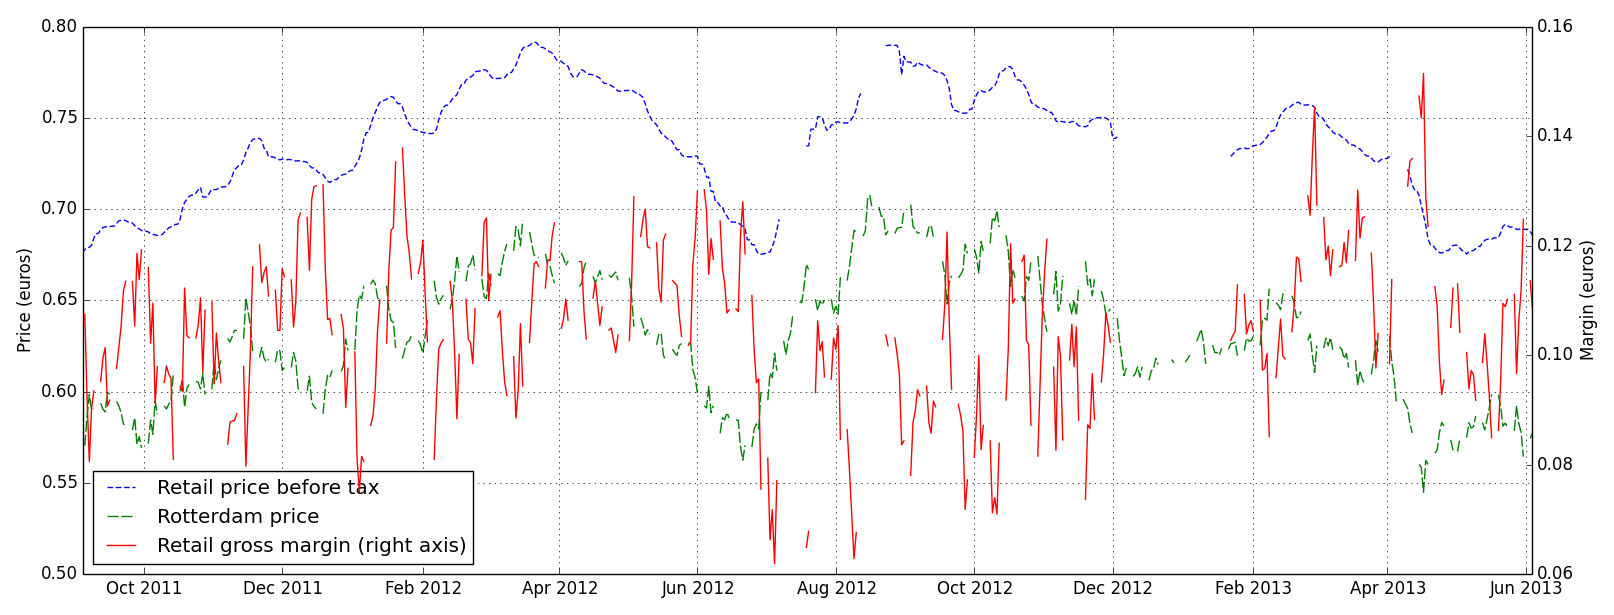
\includegraphics[width=16cm]{graphs/diesel_price_margin.png}
\end{figure}

\subsubsection{Price ridigity}

Data include prices at 9,932 gas stations in Mainland France, of which 421 are identified as highway gas stations and thus excluded from the analysis. Additionnally, 381 stations are excluded due to apparent poor data quality (less than 10 prices observed or less than a price change per month). Overall, the number of prices retained in the analysis varies between 8,715 and 8,965 across days within the period studied. On average, c. 1,500 gas stations (c. 18\% of gas stations observed and retained) change prices within a day. The average gas station changes price a little less than every week.

\begin{figure}[!h]
    \caption{Daily number of price changes (09/2011-06/2012)}
	\centering
		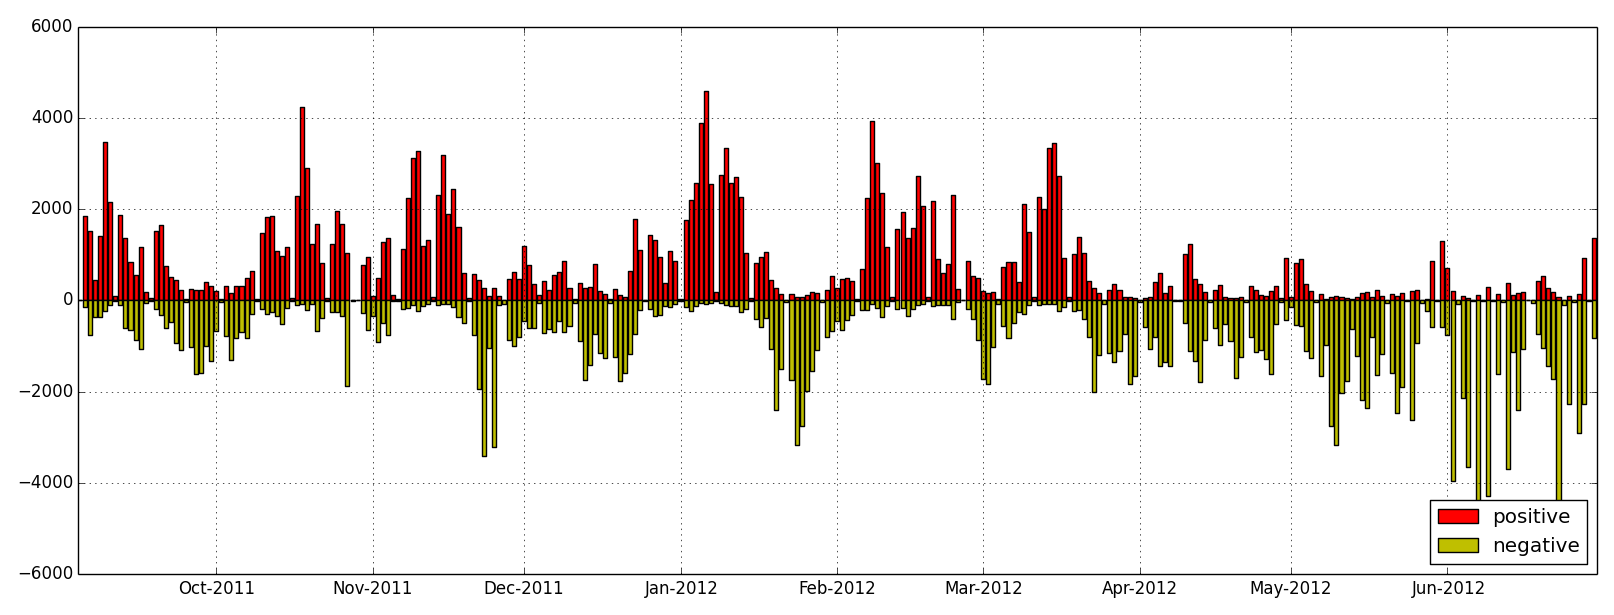
\includegraphics[width=16cm]{graphs/diesel_nb_price_chges.png}
    \floatfoot{The daily collection of prices has occasionally been delayed by a few hours resulting in some imprecision regarding the exact number of price changes occurring within one day}
\end{figure}

\subsubsection{Heterogeneity among gas stations}

Static price dispersion in French Data is easily seen in any single day price cross section. The resulting price distribution is bimodal, largely reflecting the presence of two dominant types of actors: supermarkets and oil companies. Supermarkets typically state that they use gasoline to attract customers, while oil companies mention the quality of the service to justify higher prices. Oil companies also traditionally enjoy more demand from businesses.

\section{Re-branding from "Total" to "Total Access"}

The launch of Total Access was announced by Total in a press release on September 9, 2011. The group stated its intention to develop a network of 600 gas stations through: i)the re-branding of about 300 Total gas stations, chosen based on their ability to serve the expected increase in demand (as a consequence of the decrease in price) ii) the re-branding of existing Elf gas stations (the price of which was already relatively low. The two first "prototypes" were launched in October 2011 (around Paris: which ones?). On December 16, 2013, Total reported that the 600 objective had been reached (300 end of 2012), and that 150 additional conversions were now intended.
TODO: Add details from press releases + Figaro...

\section{Impact on competition}

TODO: describe impact on competitors' prices

\section{Conclusion}

\newpage

\bibliography{references}

\newpage

\appendix

\section{Maps}

\end{document} 